\chapter{Technology Review}

\begin{figure}[h!]
	\caption{AF Date Control Logo}
	\label{image:AF-Date-Control}
	\centering
	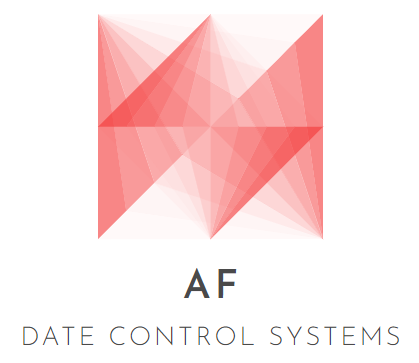
\includegraphics[width=0.50\textwidth]{images/AF-Date-Control.png}
\end{figure}

\subsection{The How and Why}
\begin{figure}[h!]
	\caption{Quotation From: https://www.brainyquote.com/}
	\label{image:quote1}
	\centering
	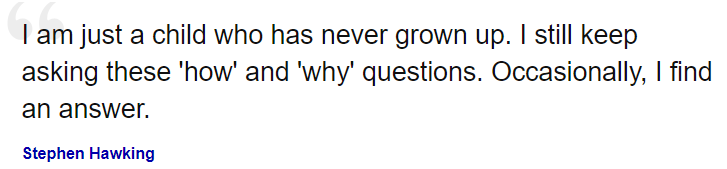
\includegraphics[width=0.8\textwidth]{images/quote1.PNG}
\end{figure}

With new ideas comes an influx of questions, the main two being the how and the why. How this idea came about ? this idea came about after five years of working part-time in retail. Looking at the day to day operations of the shop and what can be done to try and improve with what was learned in college for four years, in this case I was able to highlight one area of the shop that could be integrated into the final year project and that is to develop an application to ease the burden of Date Checking for fellow staff members. The human eye cannot spot everything, this would save time and money for the staff and shop as a whole respectively. The good thing also about this idea is the fact that it can be very flexible and can be made into various different types of applications with minor tweaks. This is a major characteristic that companies and retailers demand, versatility. It can help in many different ways.
\newline

So why this particular application and why would it be purposeful in the industry of retail. This interesting piece \cite{gustavsson2011global} provides incentive information about the global food wastage problem, this application will address this issue not just locally but globally. This piece proves it is an issue worldwide and with this application can hopefully be a massive help in reducing this worrying statistic and flatten the curve of this problem as food wastage is still on the rise. This will help staff in finding the products before they go out of date and take action. Be it reducing that particular item or using that product for something in the shop, for example identifying a packet of sausages or rashers and putting giving them to the deli staff to cook and sell in the hot deli. This is a norm in the shop where I currently work in part time and the feeling is that this is making a difference however more can be done like always. Of course you are not going to be able to give every product close to it's sell by date to the deli or reduce it. This isn't going to solve the issue entirely but to help it as much as it can. 

\subsection{Beneficial and Sufficient}
Before pursuing a Date Control Application for Retail, it needed more clarity in terms of it being beneficial to staff members and superiors in the workplace. A minor survey was conducted enclosed within the workplace to get some feedback for this potential idea. The results of this survey are in the System Evaluation section. I personally believe this application idea will be very beneficial and sufficient for retailers across the country and even beyond and the good thing about this application is that it is not intense or in anyway complicated it is basic and easy to use for the staff member or user. It is not made to look exquisite it is made to solve or help an global issue in food wastage and to save shops time and money.
\newline

Outside of retail can this be beneficial and sufficient to other industries or organisations ? very much so. It can be beneficial to the likes of charities and food banks. Items that may not be eligible for returns for credits can be donated to food banks or charities or even compost companies. \cite{riches1986food} Here is an interesting read on food banks and the welfare crisis in which it looks at the benefits of food banks for society. This is one of the many reasons why food wastage is a global issue that hopefully this basic but sufficient application can address and aid in diluting these issues. 
\newline

\begin{figure}[h!]
	\caption{CBE Provides Shop Databases and Tills}
	\label{image:cbe}
	\centering
	
\includegraphics[width=0.35\textwidth]{images/cbe.jpg}
\end{figure}

The purpose of this application other than helping the retailers directly is offering this idea or application to the local retail database and till provider known as CBE. They control the inventory of the shops and provide the retailers with modern day tills all across Connacht. Having five years experience with their system knowing that they don't offer the idea that I am trying to implement. This can prove in being very beneficial and sufficient to them in saving them time and money and providing an extra service to their new and existing customers. 
\newline

Here are some images on the permission of my superiors of the CBE Database system of where the stock is recorded as waste or returns:

\begin{figure}[h!]
	\caption{CBE's System in the workplace 1:}
	\label{image:mace1}
	\centering
	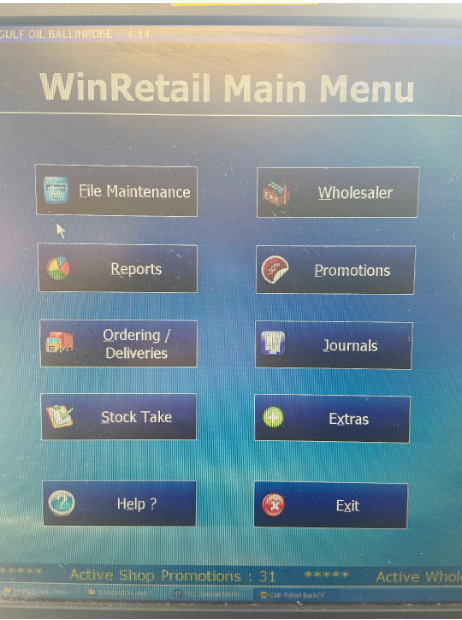
\includegraphics[width=0.5\textwidth]{images/mace1.PNG}
\end{figure}

\begin{figure}[h!]
	\caption{CBE's System in the workplace 2:}
	\label{image:mace2}
	\centering
	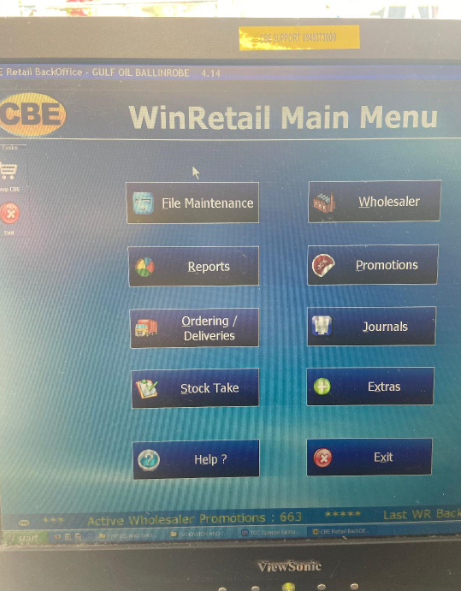
\includegraphics[width=0.56\textwidth]{images/mace2.PNG}
\end{figure}

\begin{figure}[h!]
	\caption{CBE's System in the workplace 3:}
	\label{image:mace3}
	\centering
	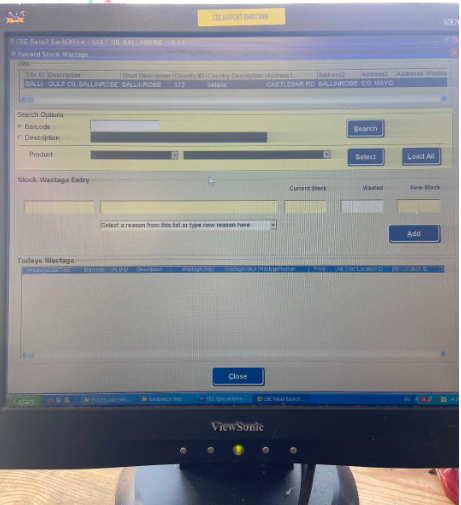
\includegraphics[width=0.57\textwidth]{images/mace3.PNG}
\end{figure}

\begin{figure}[h!]
	\caption{CBE's System in the workplace 4:}
	\label{image:mace4}
	\centering
	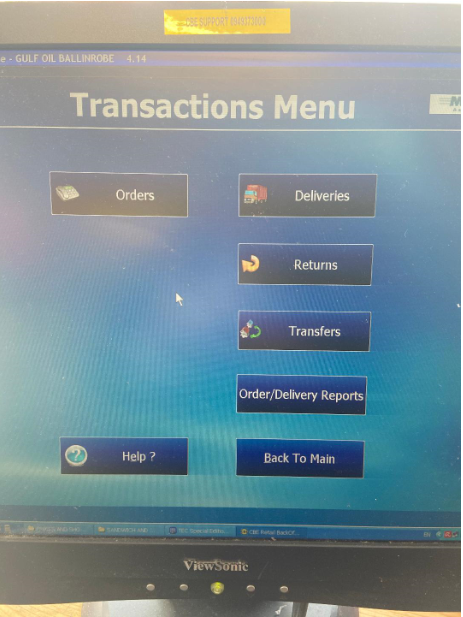
\includegraphics[width=0.51\textwidth]{images/mace4.PNG}
\end{figure}

\begin{figure}[h!]
	\caption{CBE's System in the workplace 5:}
	\label{image:mace5}
	\centering
	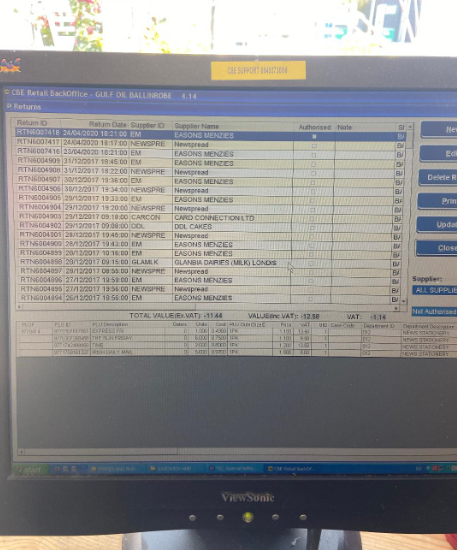
\includegraphics[width=0.55\textwidth]{images/mace5.PNG}
\end{figure}
\newpage

As you can see in the images above, this is an example taken from the shops CBE database. The system provided by CBE that gives reports, wastage, returns details and so on. You can also enter in the delivery dockets here to keep track of your stock but the implementation and presence of Date Control is not here. As humans we are expected to find the products that are close or past their sell by date, customers may have a better eye than us and find products that we missed and purchase them deeming them ineffective or dangerous for consumption. This application helps address this existing issue and prevents customer harm and helps the retailers save money and being able to act quickly. To conclude this application is beneficial and sufficient and based on the survey results, fellow staff members and superiors also think so. 

\subsection{Minor Survey}
In order to prove the idea of implementing a Date Control Application into the workplace is a good idea and will benefit and not hinder staff members, a short survey was conducted, as you can see below.

\begin{figure}[h!]
	\caption{Short Survey for Colleagues at work.}
	\label{image:survey}
	\centering
	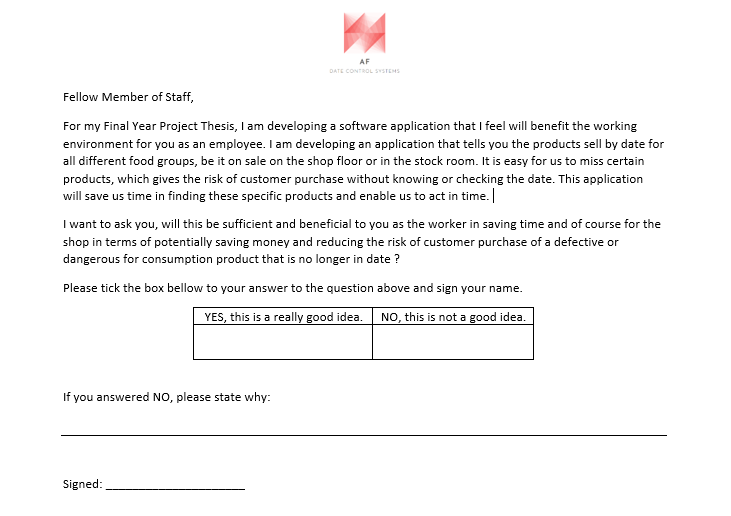
\includegraphics[width=0.8\textwidth]{images/AF-Date-Control-Survey.PNG}
\end{figure}

This is a second opinion that will influence in creating this application. Hearing different opinions being positive or negative is always good. Even if a negative response is given, it will highlight the pros and cons of this application in a more controlled environment. Does that person think it will benefit them, are they a fan of technology, they may prefer physically looking themselves rather than using an application to find things even if it may take longer in which in creating this application I am trying to save my fellow staff members time with the implementation of this application into the workplace, however everyone is entitled to their opinion. 
\newline

This was a major factor in the making and outcome of the application as it gave me more information on what to implement and not implement. This application needed to be easy to use and understand and to make the application functionality not too complex, making it quick and easy to use for staff and managers. This survey helped in getting a second opinion from someone working in the same role as me. Opinions came from fellow students and the project supervisor which were relevant but to get feedback from those who will mainly be using this application was vital in the making of this application and to get an opinion from those who will be using it.
\newline

The results from this survey are in the System Evaluation section of this dissertation. 

\subsection{Planning The Project}
The Planning of this project took place in the first semester for final year where we were told who our project supervisors would be. Once we were told who our supervisors would be it was agreed upon to meet with the designated supervisor once a week. I am in full support of the provision of supervisors for the Applied Project and Minor Dissertation as it benefited hugely in the planning of this project. 
\newline

For the first couple of weeks of meetings with the supervisor I had a few different ideas. One of them was a Date Control Application which was eventually decided upon. The other two was to make a more sufficient and more operational version of the group project done  in third year which was an Ionic Firebase application and a game in C Sharp. The Date Control Application stood out from the offset and the weeks that followed. After many discussions in person and via email it was decided to take up this project as the final year project. When this was decided a decision needed to be made on what technology that was going to be used and the research to find out has this type of application been done before or similar. 
\newline

After thorough research on the topic I came to the conclusion that this type of application was not done before or if it was it was done by someone as a minor or private application. Discussions of the prospect of introducing this idea to CBE took place once near completion as not only would it benefit retail it would benefit a company that provides shops with their tills and store databases of stock to potentially link my application in some form to their system to save them time and money and even gain customers through this latest potential technology. 
\newline

Contact was made with colleagues and superiors at the workplace to get their view on the idea of using an application to help them get stock before it's sell by date and take action and catch everything in the store, be it shop floor stock or back stock where the human eye may not catch. Knowing from experience this is an existing issue, I have missed products in the shop that my colleague might find the next day. A minor survey was conducted within the workplace and the results where then put into a pie chart which you will see in the System Evaluation section of this write up. 
\newline

The next phase of planning was to decide on what technology to use to develop this program. Due to the experience of using Firebase for the first time in third year an easy decision was made to go with Firebase as a database host for the project. Having done Ionic Firebase in third year for the end of year group project there I wanted to try something else. So I decided to go with Angular Firebase. Lucky enough for there is a range of different tutorials on Angular Firebase. This decision was made over the festive holiday period where I decided on the language choice and started sketching some ideas of how the application should look and what pages/components to implement into the application. 
\newline

I wanted to implement some elements to the application that may not be present in a CBE add on application or store application. User Authentication was one element that implemented for thesis purposes that would maybe not be on a CBE application for various reasons such as time for the staff member to register an account or sign into an account, this applications purpose is to save time for staff not hinder them. Also implementation of a product details form due to the limitation of not having a shops database at my disposal, this is included in this application to indicate the purpose of the application. To show product details and when their best before date is. So in terms of a real life situation, User Authentication and a product form wouldn't need to be required for the purpose of this idea. 
\newline

The plan to use Angular Firebase had to change in the early stages of software development for this project. The decision was made to switch to Ionic Firebase. There are various similarities between Angular and Ionic but I felt more comfortable with Ionic than Angular and not to mention liking the end product of an Ionic application rather than Angular. Thankfully the plan changed at the early stage of development.

\subsection{Technologies}
The Technologies used to develop the idea were as follows:
\newline

\begin{figure}[h!]
	\caption{Developed the code in Visual Studio Code.}
	\label{image:vscode}
	\centering
	
\includegraphics[width=0.4\textwidth]{images/vscode.png}
\end{figure}

- Visual Studio Code - The Editor of choice for coding the project.
\newline
Whenever we received a project from a lecturer, the initial thought was would it be possible to develop this project in Visual Studio Code. Out of all the editors used throughout the four years of study this stands out as the favourite. It is so easy to use and having using it for past projects and the Ionic Firebase project from third year no editor came to mind but Visual Studio Code. The file views and the smoothness of the editor when developing a program is very likeable. To develop this project I'd open a command prompt inside the project repository directory and type "code ." and it would open up the project in Visual Studio Code. This can be done with any project. It is the more favoured editor among fellow students. 
\newline

\begin{figure}[h!]
	\caption{Programming Language of choice for SD.}
	\label{image:ionic}
	\centering
	
\includegraphics[width=0.5\textwidth]{images/ionic.png}
\end{figure}
Ionic - The programming language in which the project was coded. For  the four years of software development course in GMIT I studied various different languages such as Java, C++, C, C Sharp, Python, Ruby and many more. Initially I decided to go with using Angular as my programming language for the final year project, however it was giving various issues and I didn't like the way it was turning out so a change of mind was made to code this project using the Ionic programming language framework. \cite{cheng2018build} Here is an in depth description of building an Ionic Firebase application that I came across in third year that helped with getting the project started.
\newline

Ionic enables you to develop applications using web technologies and languages like HTML, CSS, JavaScript, Angular, and Typescript. Consider Ionic as a front-end software development kit (SDK) for creating a blend of applications. Ionic provides a collection of components that imitate the native look, feel and functionality of each platform, mainly known for mobile applications but also considered for web applications also, the flexibility of Ionic Framework is why the decision was made to switch and the fact that  it suits what I in-visioned when sketching the pages and how they look for the user. Examples of these components include buttons, tabs, menus, lists, cards, modals, and so on. However for colors it is not so broad, but they suited what I was trying to implement. At the end of the day this application was not created to look pretty it was created to solve a problem in the work place, a Date Control Problem.
\newline
\newpage
Out of the four years of studying software development, Ionic and Angular stood out. In the second year of study in GMIT I encountered the Angular Framework, and in third year encountered the Ionic Framework. When coming up with the idea of creating my Date Control application the choice was to pick a language I liked and enjoyed coding. In third year for the group project myself and another student created a cinema booking website using Ionic Firebase. From then I wanted to use Firebase for its easy implementation into the Ionic Framework for an application. As always wanting to learn something new, although similar Ionic and Angular are different, as mentioned above initially started the project in Angular and then switched to Ionic. This was done as I did not feel as comfortable with Angular Firebase as I did with Ionic Firebase. I'm glad the switch was made for a number of reasons including software development, overall design and it's link to the Firebase DB Cloud.
\newline

\begin{figure}[h!]
	\caption{Cloud Database of My choosing for Data Storage.}
	\label{image:fire-base}
	\centering
	
\includegraphics[width=0.5\textwidth]{images/fire-base.png}
\end{figure}

- Firebase - The Cloud Database used for this application to store User Authentication details and store the product entry data for crud functionality. Note for private and security purposes the admin of the Firebase database cannot see what the users passwords are, Firebase hash them in which I or anyone else does not know. Within Visual Studio Code in the software development to connect the Firebase database project made on Firebase implementation of a  unique Firebase configuration values to the environments files. It should look something like this if you were to ever take up a project with Firebase.   
\newline

\begin{figure}[h!]
	\caption{Example of Firebase Configuration:}
	\label{image:firebaseConfig}
	\centering
	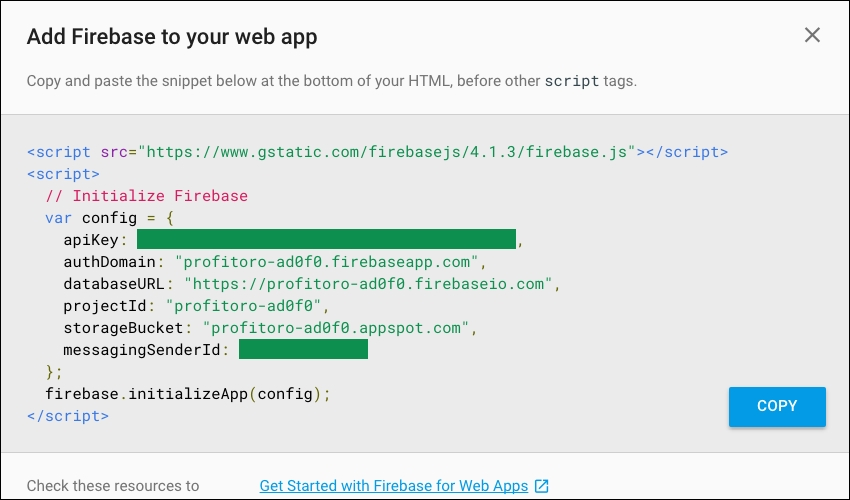
\includegraphics[width=0.5\textwidth]{images/firebaseConfig.jpg}
\end{figure}

\begin{figure}[h!]
	\caption{All Project Items are on GitHub and can be cloned.}
	\label{image:github1}
	\centering
	
\includegraphics[width=0.4\textwidth]{images/github.png}
\end{figure}
\newpage
- GitHub - Used to publish the project on the internet for the thesis and for people to then test themselves. GitHub gives a brief description of the project as a whole and explains to the person wishing to test how to run or try out the application. 
\newline

\begin{figure}[h!]
	\caption{This project dissertation was edited on Overleaf in LaTeX.}
	\label{image:overleaf-latex}
	\centering
	
\includegraphics[width=0.4\textwidth]{images/overleaf-latex.png}
\end{figure}
- Overleaf - Used overleaf as a Latex editor for this project dissertation. Used this template provided to us from our year head. Only came across Overleaf with LaTeX in the first semester of final year where much like this section we needed to create a Literature review. This benefited in terms of writing this dissertation.

\subsection{Issues}

\begin{figure}[h!]
	\caption{In Every Project or Idea Issues arise.}
	\label{image:issues}
	\centering
	
\includegraphics[width=0.58\textwidth]{images/issues.jpg}
\end{figure}

In every project or idea issues can very easily arise. During the software development you may encounter issues such as compile errors, server errors, and maybe some code implemented that worked on older versions of software, for example, some functions or declarations that work on Ionic 2 wont work on Ionic 5 and so on. HTML issues such as buttons not working, pages not showing due to an error in the code and so on. Issues can very easily arise in any software projects, in fact make that any project whatsoever. In this section I will be discussing the issues that arose for me during the software development part of the project. 
\newline

The first issue arose when pursuing the Date Control Application in Angular Firebase. Having done Ionic Firebase in Third Year for the group project the sense of a challenge was there in trying out Angular with Firebase. Having set up the authentication with Angular Firebase, the way it was looking and what it was going to look like when implementing the CRUD functionality to the application was not what the vision looked like. In the end it was the correct decision in the long run. I referenced the third year project a lot during the making of this application as it too was Ionic Firebase. In terms of experience this worked in my favour. 
\newline

The realisation hit that pursuing this project in Ionic would be the best option. The switch was made which you can see in the early commits of the software development of the project. The switch was made of course for the reasons mentioned, however the switch also came due to the fact of being familiar with Ionic Firebase having completing a project in it before. The overall look of Ionic intrigued me. This did not hinder to much in the completion of this application. When the switch was done it was at the stage of testing the waters, what will and won't work and how it will look in the end. This wasn't a major issue and the switch was the correct decision. 
\newline

The Next issue that arose was the authentication "reset/forgot" password. After looking at many different tutorials online I was unable to get this function to work. The code is still in the project directory but has to be commented out due to "ionic build" errors when trying to make the project a Firebase hosted website. Due to the fact if CBE were to implement this application into their systems they may not have the idea of a user authentication system within it, as this is a prototype it does not hinder the overall reasoning for this application. A password reset email can be sent via the Firebase console to the user upon request. This issue is highlighted in the issues section of the GitHub Repository for this project.
\newline

Another issue that stood out was the sorting issue. I wanted to sort the data read into the Firebase Cloud Database to be loaded into the food groups pages with the best before date closest to the current date to be at the top of the list. Unfortunately this feature was not implemented. Various different ways were tried to implement it such as a query in the get product details function and also the fetch product details functionality that shows the product details on the page. Attempts were also made to alter the Firebase database to show this by trying to implement rules to do so. I was unable to make this feature work, however the idea was there and may be implemented if taken up by the likes of CBE who may take a different approach in showing data in this format. This issue is highlighted in the issues section of the GitHub Repository for this project.
\newline

A Small bug started to arise when signing into an account also. Where a window pop up gives an error message along the lines of "null is not an object". This issue is also highlighted on GitHub. This does not hinder a sign in, as if you click the log in button again it will sign you in.
\newline

Thankfully no major issues arose that were expected to arise, for example when making this application a Firebase hosted website the fear was present of when trying to do this will result in the application breaking completely. Since this was at a late stage it was a very fragile time in the software development phase. 

\newpage
\subsection{Technology References}
\url{https://developer.okta.com}
\newline
\url{https://ionicframework.com/docs/theming/colors}
\newline
\url{https://ionicframework.com/docs/building/running}
\newline
\url{https://www.tutorialspoint.com/ionic/ionic_colors.htm}
\newline
\url{https://ionicons.com/}
\newline
\url{https://www.youtube.com/watch?v=M-nTpVIyGw0}
\newline
\url{https://devdactic.com/host-ionic-website-firebase/}
\newline
\url{https://forum.ionicframework.com/t/how-to-add-styles-to-ion-button-inner-text/148987}
\newline
\url{https://ionicframework.com/docs/native/firebase-authentication}
\newline
\url{https://www.freakyjolly.com/ionic-firebase-crud-operations/#.XrKlWqhKjIU}
\newline
\url{https://github.com/AndreasFahey/ajproject}

